\documentclass{article}
\usepackage[utf8]{inputenc}
\usepackage{enumerate}
\usepackage{graphicx}

\title{Module Guide\\
Dragon Age}
\author{Group 8: Team Eight \\
                 Stanley Liu (MacID: liuz23) \\    
                 Toni Miharja (MacID: miharjat)\\
                 Zhi Zhang (MacID: zhangz1)}
\date{November 10 2017 }
\usepackage[showgrame]{geometry}

\usepackage{titling}
\renewcommand\maketitlehooka{\null\mbox{}\vfill}
\renewcommand\maketitlehookd{\vfill\null}

\begin{document}
\maketitle
\newpage
\tableofcontents
\newpage
 
\section{Revision History}
\begin{table}[!htbp]
	\begin{tabular}{|l|l|1|1|}
		\toprule
		\hline
		Date & Author & Notes & Version\\ \hline
		November 7, 2017 & Toni & Introduction & 1.0\\ \hline
		November 8, 2017 & Stanley & Anticipated and Unlikely Changes, Module Decomposition & 1.1\\ \hline
		November 8, 2017 & Toni & Use Hierarchy between Modules & 1.2\\ \hline
		November 9, 2017 & Toni, Stanley & Module Decomposition & 1.3\\ \hline
		November 10, 2017 & Toni, Stanley & Traceability Matrix, Module Decomposition & 1.4\\ \hline
		
	\end{tabular}
	\caption{Revision History: Module Guide}
\end{table}

\section{General Information and Introduction}
This document serves as the Module Guide (MG) and Design Documentation for our Dragon Age (DA) Project. This document will be useful for the following target audience:
\begin{itemize}
    \item New Project Contributors: New members can quickly get up to speed by understanding the big picture of the project as they read this document.
    \item Developers/ Designers: This document will be the central collection of documentation for designers and developers with detailed explanation of module specifications. It also helps the designers in determining if the product design will satisfy the requirements of the program, allowing for a traceback to the requirements.
    \item Maintainers: Under the anticipated changes section, maintainers will be able to design future alterations without severely affecting the rest of the modules by understanding the program architecture. They will also be able to plan ahead as they roll out improvements and changes to the next versions.
\end{itemize}
\subsection{Modular Decomposition}
The team acknowledge the importance of decomposing a system into modules and further into sub-modules as it is a crucial task to ensure that the large system is easily maintained, coded and understood. Modular decomposition prevents the system from becoming too complicated as it grows. By doing so, it allows multiple developers to concurrently develop components while minimising the risk of “breaking” the project. A highly modular system will allow new features to be added seamlessly without much alterations to the current working environment.
\subsection{Document Organization}
The rest of the document is organised in the following manner:
\begin{itemize}
    \item Section 3 lists the anticipated and unlikely changes of the software requirements.
    \item Section 4 summarizes the module decomposition that was constructed according to the likely changes.
    \item Section 5 specifies connections between the software requirements and the modules. 
    \item Section 6 gives a detailed description of the modules.
    \item Section 7 includes one traceability matrices. It shows the relation between anticipated changes and the modules.
    \item Section 8 specifies the Uses Relationship, describing the use relation between modules.
\end{itemize}

\section{Anticipated and Unlikely Changes}
 This section lists some possible changes that may occur to our project. Anticipated changes are in section 3.1 and unlikely changes are in section 3.2.
 \subsection{Anticipated Changes}
 Anticipated changes are the changes that will be made to elements that hide in modules, and are easy to change without affecting the rest of the project.\\\\
\textbf{AC1}: More game controls (ex: keyboard shortcuts for user’s convenience)\\
\textbf{AC2}: Sound features of the game\\
\textbf{AC3}: Additional functionalities (ex: additional dragon type or enemy type)\\
\textbf{AC4}: Images of the components of the game (map, dragons, buttons)\\
\subsection{Unlikely Changes}
Unlikely changes are the design decisions that affect the main components and functions of the game. In risk of having to modify multiple modules of the game, these decisions are unlikely to change.\\\\
\textbf{UC1}: The main goal of the game: the concept of defending base from enemies using attacking units\\
\textbf{UC2}: The programming language: Python and Pygame\\
\textbf{UC3}: The game controller: mouse\\
\textbf{UC4}: The input data (database of dragons and enemies), not including images\\

\section{Module Hierarchy}
\begin{table}[!htbp]
	\begin{tabular}{|l|l|}
		\toprule
		\hline
		Level 1 & Level 2\\ \hline
		Hardware Hiding Module & \\ \hline
		Behaviour Hiding Module & \vtop{\hbox{\strut M1. Dragon Tower Module}\hbox{\strut M2. Timer Bullet Module}\hbox{\strut M3. Timer Enemy Module}\hbox{\strut M4. Timer Hover Module}\hbox{\strut M5. Timer Fired Module}\hbox{\strut M6. Draw Module}\hbox{\strut M7. Game Manager Module}\hbox{\strut M8. Dragon Age Module}}\\\hline
		Software Decision Hiding Module & \vtop{\hbox{\strut M9. Dragon Module}\hbox{\strut M10. Enemy Module}\hbox{\strut M11. Bullet Module}\hbox{\strut M12. Path Module}\hbox{\strut M13. Game Date Module}}\\\hline
	\end{tabular}
	\caption{Module Hierarchy}
\end{table}

\section{Connection Between Requirements and Design}
The system is designed to satisfy the requirements developed in the System Requirement Specification document. In this document, the system is decomposed into modules that ultimately meet the requirements specified.
\section{Module Decomposition}
\subsection{Hardware Hiding Modules}
\textbf{Secret:}The implementation of the interpreter\\
\textbf{Services:}This module serves as the interface between the game and the hardware. It allows the system to communicate with the the code\\
\textbf{Implemented By:}Python interpreter and Operating System\\

\subsection{Behaviour-Hiding Module}
\textbf{Secret:}Behaviours\\
\textbf{Services:}This module describes the visible behavior of the game. It functions as the interpreter between hardware hiding modules and software decision modules\\
\textbf{Implemented By:}N/A\\

\subsubsection{Dragon Tower Module}
\textbf{Secret:}Dragon Tower\\
\textbf{Services:}The dragon tower checks if enemies are in range and shoots at enemies\\
\textbf{Implemented By:}Python Library\\

\subsubsection{Timer Bullet Module}
\textbf{Secret:}Move and remove bullets\\
\textbf{Services:}Get the Dragon Towers to fire the bullets to enemies\\
\textbf{Implemented By:}Python Library\\

\subsubsection{Timer Enemy Module}
\textbf{Secret:}Move enemy\\
\textbf{Services:}Waves of enemies move into the map following the path\\
\textbf{Implemented By:}Python Library\\

\subsubsection{Timer Hover Module}
\textbf{Secret:}Hover display\\
\textbf{Services:}Display a rectangle of size of dragon when player selects the dragon and hovering the dragon on board\\
\textbf{Implemented By:}Python Library\\

\subsubsection{Timer Fired Module}
\textbf{Secret:}Timer Fired\\
\textbf{Services:}Initiate all timer fired functions\\
\textbf{Implemented By:}Python Library\\

\subsection{Draw Module}
\textbf{Secret:}Draw objects\\
\textbf{Services:}Draw every game object onto the pygame window\\
\textbf{Implemented By:}Python Library\\

\subsubsection{Game Manager Module}
\textbf{Secret:}Manage game data\\
\textbf{Services:}Initiates all game data\\
\textbf{Implemented By:}Python Library\\

\subsubsection{Dragon Age Module}
\textbf{Secret:}Run the game\\
\textbf{Services:}Initiates pygame\\
\textbf{Implemented By:}Python Library\\

\subsection{Software Decision Module}
\textbf{Secret:}Data Structure\\
\textbf{Services:}Provides the data structure to store information from the game\\
\textbf{Implemented By:}N/A\\

\subsubsection{Dragon Module}
\textbf{Secret:}Dragon Party\\
\textbf{Services:}Dragon objects are created and are appended to the dragon party list for players to use\\
\textbf{Implemented By:}Python Library\\

\subsubsection{Enemy Module}
\textbf{Secret:}Enemy Wave\\
\textbf{Services:}Create enemy object and append enemies into enemy wave list\\
\textbf{Implemented By:}Python Library\\

\subsubsection{Bullet Module}
\textbf{Secret:}Bullet\\
\textbf{Services:}Create bullet object and set bullet attributes\\
\textbf{Implemented By:}Python Library\\

\subsubsection{Path Module}
\textbf{Secret:}Path\\
\textbf{Services:}Create enemy path\\
\textbf{Implemented By:}Python Library\\

\subsubsection{Game Data Module}
\textbf{Secret:}Game Data\\
\textbf{Services:}Set initial game data\\
\textbf{Implemented By:}Python Library\\

\section{Traceability Matrix}
The following are traceability matrices. The first trace is between the modules and the requirements specified in the requirement document. The second trace is between the modules and the anticipated changes.

\subsection{Trace Between Anticipated Changes and Modules}
\begin{table}[!htbp]
	\begin{tabular}{|l|l|}
		\toprule
		\hline
		Anticipated Changes & Modules\\ \hline
		AC1: More game controls & M7. Game Manager Module\\ \hline
		AC2: Sound features of the game & M7. Game Manager Module\\\hline
		AC3: Additional functionalities & \vtop{\hbox{\strut M9. Dragon Module}\hbox{\strut M10. Enemy Module}\hbox{\strut M11. Bullet Module}\hbox{\strut M12. Path Module}}\\\hline
		AC4: Images of the components of the game & M9. Dragon Module\\\hline
	\end{tabular}
	\caption{Trace Between Anticipated Changes and Modules}
\end{table}

\section{Use Hierarchy Between Modules}
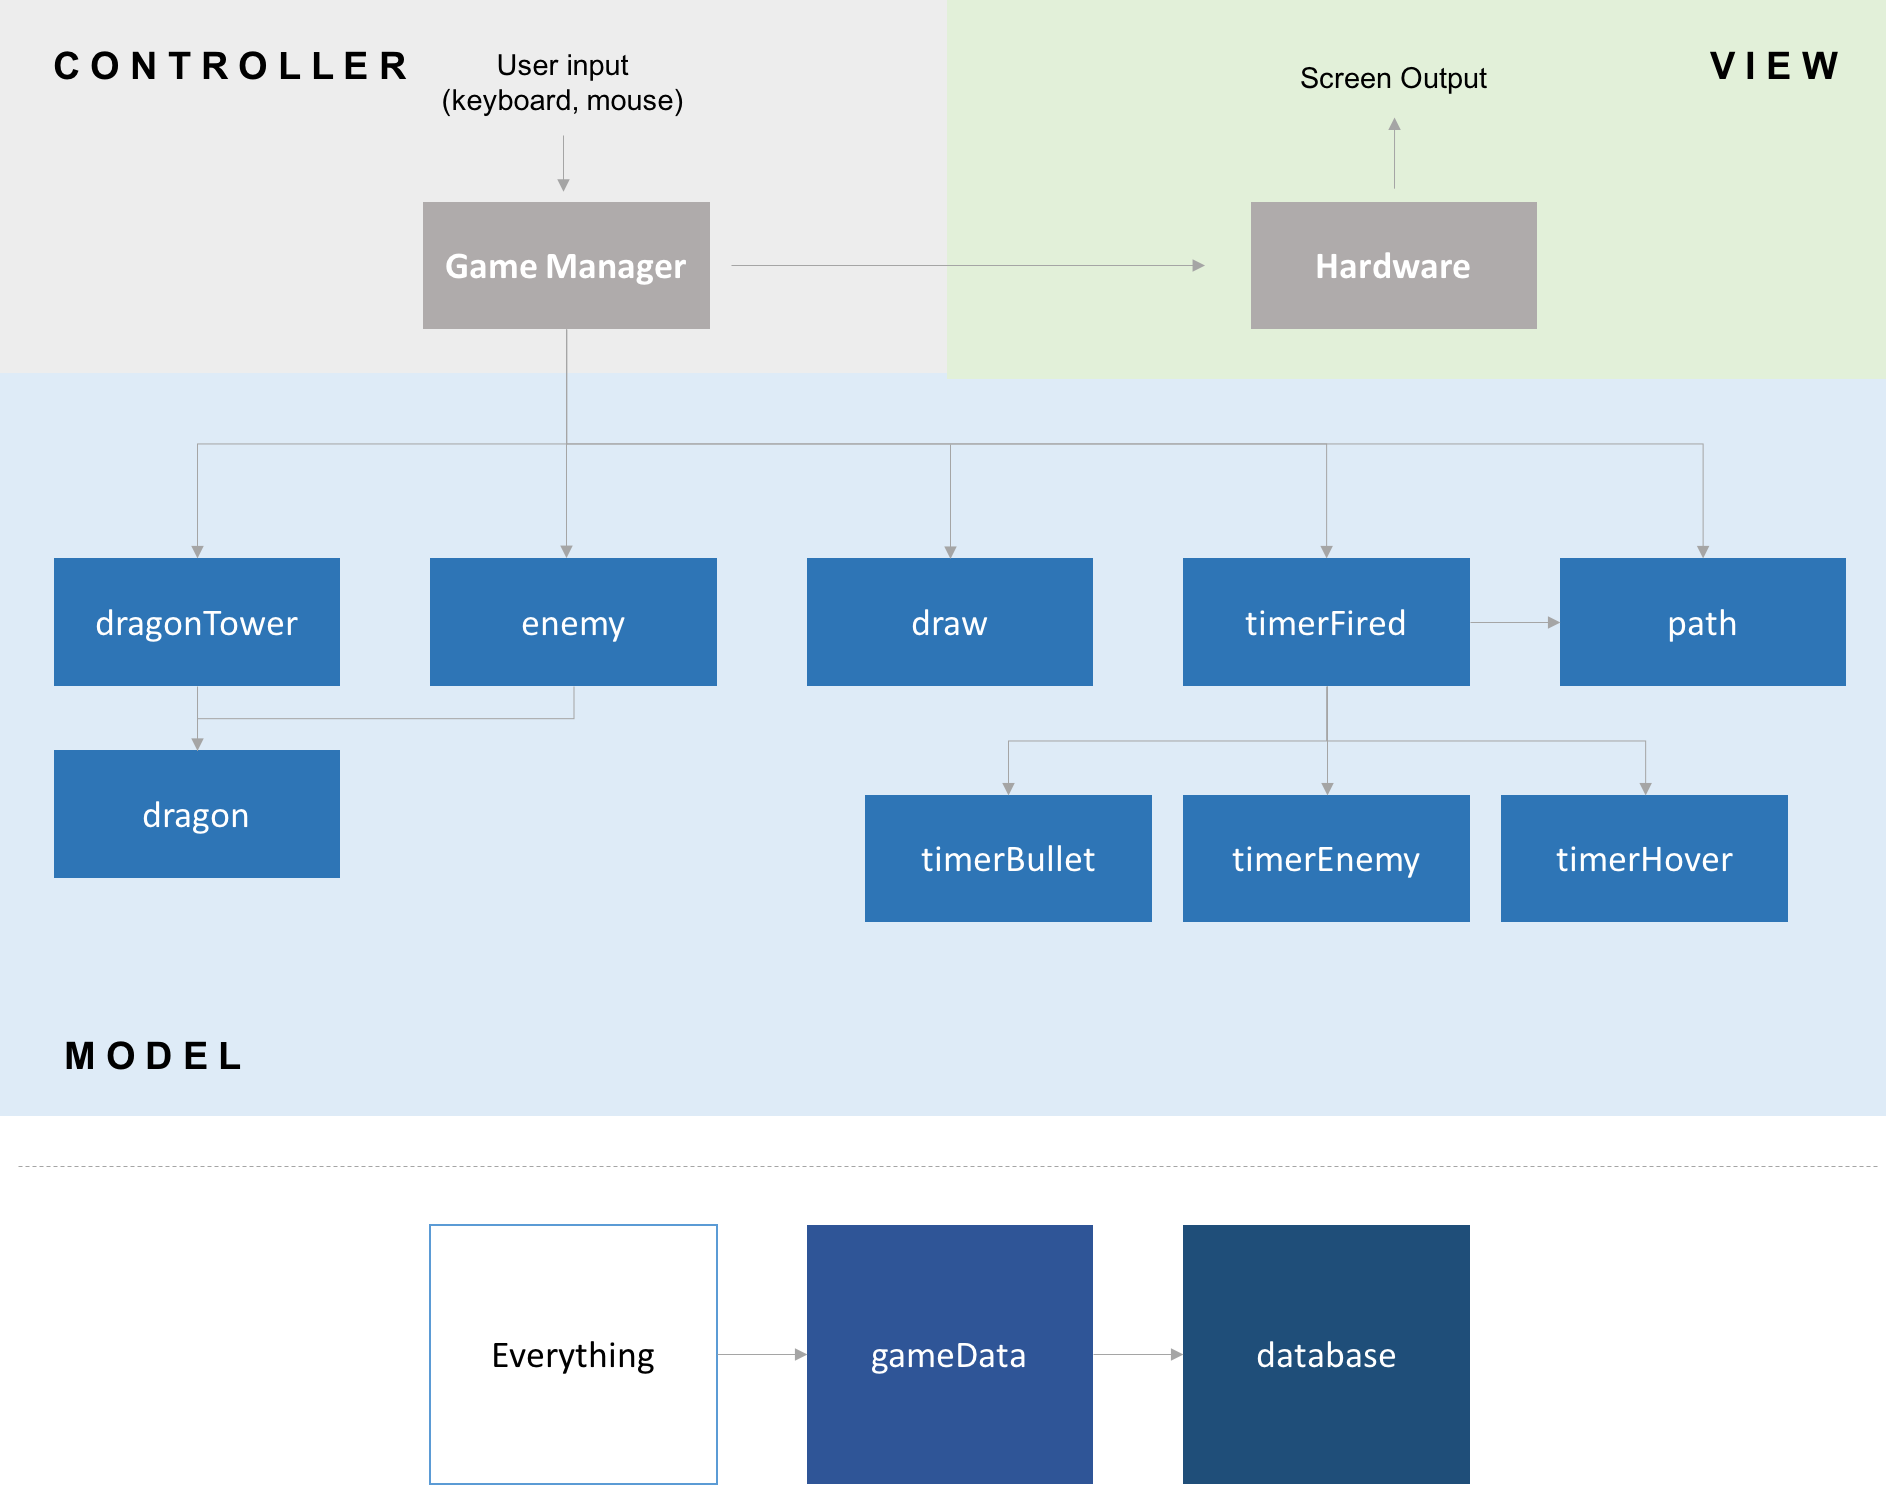
\includegraphics[scale=0.52]{UseDiagram.png}
Figure 1: Uses Hierarchy Between Modules

\section{Project Schedule}
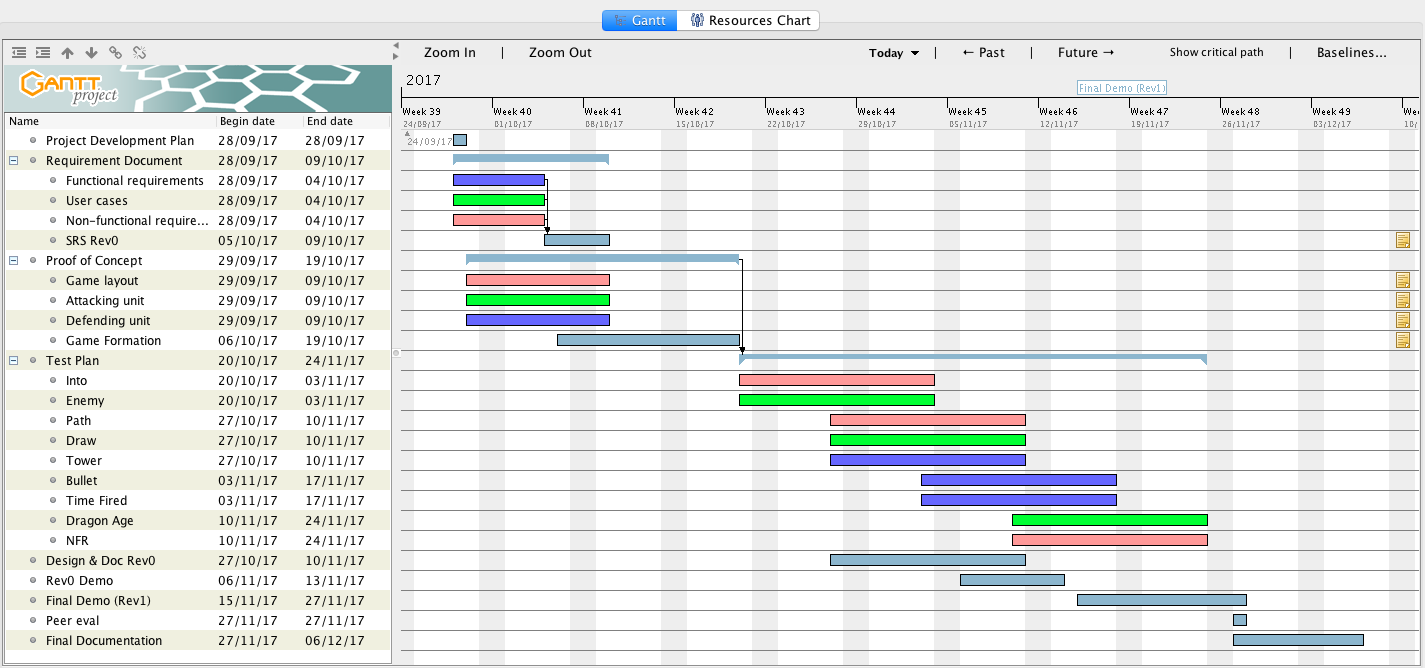
\includegraphics[scale=0.33]{gantt8.png}
Figure 2: Gantt Chart of Project Schedule

\end{document}
